\subsection{Angular controller}
The purpose of the angular controller is to have the vehicle turn according to a reference, that the controller gets from the route planning. As the steering only have a little linear area (See \appref{app:LinearAreaKp}), the types of controller that can be used is very limited. A controller type that can be used is a proportional controller.

\subsubsection{Proportional controller}

\begin{figure}[H]
  \centering
  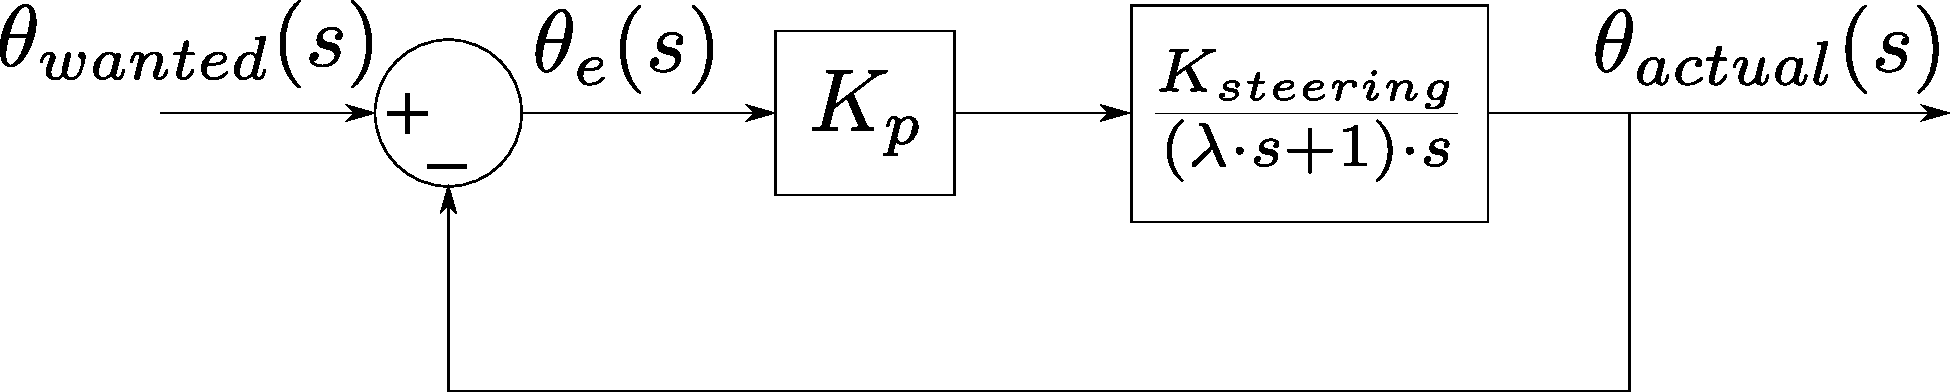
\includegraphics[scale=0.3]{figures/angularController.pdf}
  \caption{Illustration of a proportional controller for the steering.}
  \label{fig:PconAngpic}
\end{figure}

On \figref{fig:PconAngpic}, there is implemented a proportional controller into the model for the angular steering model, from \secref{sec:SteeringModel}. This will give the following closed loop transfer function:

\begin{flalign}
  \eq{ \frac{\theta_{actual}}{\theta_{wanted}} }{ \frac{\frac{ K_p \cdot K_v \cdot K_s }{ (\lambda \cdot s + 1) \cdot s } }{ \frac{ K_p \cdot K_v \cdot K_s }{ (\lambda \cdot s + 1) \cdot s } + 1} }&\label{eq:PconAng}
\end{flalign}

According to \appref{app:steeringGainTest}, the product of $K_v$ and $K_s$, called $K_{steering}$, is equal to:

\begin{flalign}
\eq{K_{steering}}{0,5149 \cdot v - 0,1925}
\end{flalign}

As $v$ is the wanted velocity, which is 1,4 $m \cdot s^{-1}$, $K_{steering}$ is equal to 0,386. And with lambda equal to the servo duty cycle time constant on 30 ms, the transfer function will be:

\begin{flalign}
  \eq{ \frac{\theta_{actual}}{\theta_{wanted}} }{ \frac{\frac{ K_p \cdot 0,386 }{ (0,03 \cdot s + 1) \cdot s } }{ \frac{ K_p \cdot 0,386 }{ (0,03 \cdot s + 1) \cdot s } + 1} }&\label{eq:PconAng2}
\end{flalign}

This is converted to the standard form:

\begin{flalign}
  \eq{ \frac{\theta_{actual}}{\theta_{wanted}} }{ \frac{1}{\frac{ 0,03 \cdot s^2 + s }{ K_p \cdot 0,386 } + 1} }&\label{eq:PconAng3}
\end{flalign}

According to \appref{app:LinearAreaKp}, the system with a proportional controller is only linear within the range of a $K_p$ on 1,5 to 3. To get smallest possible time constant, the $K_p$ need to be as big as possible. Therefore the $K_p$ is set to 3, which give:

\begin{flalign}
  \eq{ \frac{\theta_{actual}}{\theta_{wanted}} }{ \frac{1}{\frac{ 0,03 \cdot s^2 + s }{ 3 \cdot 0,386 } + 1} \Rightarrow \frac{1}{ 0,026 \cdot s^2 + 0,86 \cdot s + 1} }&\label{eq:PconAng4}
\end{flalign}

From this transfer function, it can be seen that the gain is equal to one and the system is a second order system. The reason that the proportional controller here give a gain equal to 1 and the proportional controller for the velocity does not, is that there is a integrator in this system, that removes this steady state error. This way, a proportional controller will be good enough to handle the controlling of the angular movement of the vehicle. 

The proportional controller is then implemented. For the feedback, the magnetometer is used (see \secref{sec:magnetoSensor}). For the sampling time, it have been chosen to be the same as the length of the duty cycle for servo, on 30 ms. As the magnetometer only needs to update one time, each time the controller sends a new duty cycle to the servo, there is not needed for a higher sampling frequency. The sampling frequency will then be on:

\begin{flalign}
  \eq{ f_{sampling} }{ \frac{1}{30 ms} \Rightarrow 33,33}\unit{Hz} \label{eq:PconAng5}
\end{flalign} \todo{Needs units}

The angular controller is then tested, where the start heading is \si{5^{\circ}} and the reference heading is \si{45^{\circ}}. The test is shown on \figref{fig:AngularTestSim}.

\begin{figure}[H]
 	\centering
 	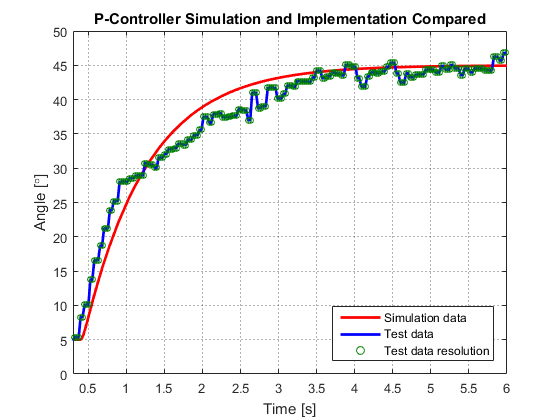
\includegraphics[width=\textwidth]{figures/SteeringAngularTest}
 	\caption{Test of the proportional controller, with a start heading on \si{5^{\circ}} and a reference on \si{45^{\circ}}.}
 	\label{fig:AngularTestSim}
\end{figure}

As shown on \figref{fig:AngularTestSim}, the system react nearly the same way as the simulation and end up at the same rise time as the simulation. 